% LaTeX Template for Project Report, Version 2.0
% (Abstracted from a Major Project Report at CSED, NIT Calicut but can be
% modified easily to use for other reports also.)
%
% Released under Creative Commons Attribution license (CC-BY)
% Info: http://creativecommons.org/licenses/by/3.0/
%
% Created by: Kartik Singhal
% BTech CSE Batch of 2009-13
% NIT Calicut
% Contact Info: kartiksinghal@gmail.com
%
% It is advisable to learn the basics of LaTeX before using this template.
% A good resource to start with is http://en.wikibooks.org/wiki/LaTeX/
%
% All template fields are marked with a pair of angular brackets e.g. <title here>
% except for the ones defining citation names in ref.tex.
%
% Empty space after chapter/section/subsection titles can be used to insert text.
%
% Just compile this file using pdflatex after making all required changes.

\documentclass[12pt,a4paper]{report}
\usepackage[pdftex]{graphicx} %for embedding images
\usepackage{url} %for proper url entries
\usepackage[bookmarks, colorlinks=false, pdfborder={0 0 0}, pdftitle={<pdf title here>}, pdfauthor={<author's name here>}, pdfsubject={<subject here>}, pdfkeywords={<keywords here>}]{hyperref} %for creating links in the pdf version and other additional pdf attributes, no effect on the printed document
%\usepackage[final]{pdfpages} %for embedding another pdf, remove if not required
\usepackage{titlesec}
\usepackage{textcomp}
\usepackage{textgreek}
\usepackage{pdfpages}
\usepackage[toc,page]{appendix}
\usepackage{ragged2e}
\usepackage{amsmath}
\usepackage{amsthm}
\usepackage[margin=1.2 in]{geometry}
\usepackage{longtable}
\titleformat{\chapter}[hang]
  {\normalfont\Huge\bfseries}{\chaptertitlename\thechapter}{1em}{}
\usepackage{graphicx}
\usepackage{amssymb}
\usepackage{epstopdf}
\usepackage{float}

\begin{document}
\renewcommand\bibname{Bibliography} %Renames "Bibliography" to "References" on ref page
\renewcommand{\chaptername}{}
\setcounter{chapter}{0}

%include other pages
\begin{titlepage}

\begin{center}

\textup{\small {\bf September 27th, 2019} \\ MScF}\\[0.2in]

% Title
\Large \textbf {Data Science For Finance \\ Exercise Session 2}\\[0.5in]

       \small \emph{Submitted in partial fulfillment of\\
        the requirements for the course of}
        \vspace{.2in}

       {\bf Data Science for Finance \\ HEC Lausanne \\ University of Lausanne}\\[0.5in]

% Submitted by
\normalsize Submitted by \\
\begin{table}[h]
\centering
\begin{tabular}{lr}\hline \\
Student ID & Names of Students \\ \\ \hline
\\
194 21 437 & Nora Koennyu \\
128 20 858 & Marceau Pierron \\
137 58 495 & David Sasselli \\ 
164 05 136 & Taulant Ukshini \\ \\ \hline 
\end{tabular}
\end{table}

\vspace{.1in}
Under the guidance of\\
{\textbf{Florian Ielpo}}\\[0.2in]

\vfill

% Bottom of the page
%\includegraphics[width=0.18\textwidth]{nitc-logo}\\[0.1in]
%\Large{Department of Computer Science and Engineering}\\
\normalsize
\textsc{University of Lausanne - HEC Lausanne}\\
Unil Internef - 1015 - Lausanne \\
\vspace{0.2cm}
Fall Semester 2019

\end{center}

\end{titlepage}

%\input{certificate}
%\input{abstract}

\pagenumbering{roman} %numbering before main content starts
%\tableofcontents
%\listoftables
%\listoffigures

\newpage
\pagenumbering{arabic} %reset numbering to normal for the main content


\chapter{Exercise 1}

\section{Question 1}

\subsection{Compute the expectation and the variance of this distribution}
\subsubsection{Expectation}

\begin{align}
    \begin{split}
        P(X=k) =& \; \frac{\lambda^k e^{-\lambda}}{k!} \;\; ; \; X \sim P(\lambda) \\ \\
        E[X] =& \; \sum_{k=0}^{\infty} k \cdot P(X=k) \\
        \Rightarrow \; E[X] =& \; \sum_{k=0}^{\infty} k \cdot \frac{\lambda^k \cdot e^{-\lambda}}{k!} \\
        \Rightarrow \; E[X] =& \; \sum_{k=1}^{\infty} \frac{\lambda^{k} e^{-\lambda}}{(k-1)!} \\
        \Rightarrow \; E[X] =& \; \lambda e^{-\lambda} \cdot \sum_{k=1}^{\infty} \frac{\lambda^{k-1}}{(k-1)!} \;\; ; \;\; \lim_{n \to \infty} \sum_{n}^{\infty} \frac{\lambda^n}{n!} = e^{\lambda} \\
        \Rightarrow \; E[X] =& \; \lambda e^{-\lambda} e^{\lambda} \\
        \Rightarrow \; E[X] =& \; \lambda
    \end{split}
\end{align}

As we can see, the estimator is the mean of the sample. The expected value of a Poisson random variable is equal to its parameter $\lambda$, therefore the sample mean is an unbiased estimator of the expected value.

\subsubsection{Variance}

\begin{align}
    \begin{split}
        P(X=k) =& \; \frac{\lambda^k e^{-\lambda}}{k!} \;\; ; \; X \sim P(\lambda) \\
        Var[X] =& \; E[X^2] - E^2[X] \\
        \Rightarrow \; Var[X] =& \; \sum_{k=0}^{\infty} k^2 \cdot P(X=k) \; - \lambda^2 \\ \\
        E[X^2] =& \sum_{k=0}^{\infty} k^2 \cdot \frac{\lambda^k \cdot e^{-\lambda}}{k!} \\
        \Rightarrow \; E[X^2] =& \; \lambda e^{-\lambda} \cdot \sum_{k=1}^{\infty} k \cdot \frac{\lambda^{k-1}}{(k-1)!} \\
        \Rightarrow \; E[X^2] =& \; \lambda e^{-\lambda} \cdot \left( \sum_{k=1}^{\infty} (k-1) \frac{\lambda^{k-1}}{(k-1)!} + \sum_{k=1}^{\infty} \frac{\lambda^{k-1}}{(k-1)!} \right) \\
        \Rightarrow \; E[X^2] =& \; \lambda e^{-\lambda} \cdot \left( \lambda \cdot \sum_{k=1}^{\infty} \frac{\lambda^{k-2}}{(k-2)!} + \sum_{k=1}^{\infty} \frac{\lambda^{k-1}}{(k-1)!} \right) \;\; ; \;\; \lim_{n \to \infty} \sum_{n}^{\infty} \frac{\lambda^n}{n!} = e^{\lambda} \\
        \Rightarrow \; E[X^2] =& \; \lambda e^{-\lambda} \cdot (\lambda e^{\lambda} + e^{\lambda}) \\
        \Rightarrow \; E[X^2] =& \; \lambda^2 + \lambda \\ \\
        \Rightarrow \; Var[X] =& \; \lambda^2 + \lambda - \lambda^2 \\
        \Rightarrow \; Var[X] =& \; \lambda
    \end{split}
\end{align}

Again, the variance of a Poisson random variable is equal to its parameter $\lambda$ [blablabla efficiency bla....]

\section{Question 2}
There are several reasons, first of all $\lambda$ is the only parameter we need to define the Poisson distribution, once $\lambda$ is known then mean and variance follow effortlessly as seen in the previous exercise.
The Poisson distribution also possess another interesting and useful property: the Markov property (memorylessness). In probabilistic forecasting is a desirable property that may enable a simplified way to the solution of complex problems.[...]
The estimator $\lambda$ distributes exactly like a Poisson distribution with parameter n$\lambda$. This distribution, for a sufficient big n can be approximated by the Normal distribution with same average and variance as the relative Poisson distribution.

\section{Question 3}
As shown in the plot, the distribution is centered on 0.5 and we clearly see the impact of the number of observations on the 4th momentum (Kurtosis). In fact, the more the observations, the more efficient our estimator becomes, resulting on a peak in the density plot.
\section{Question 4}
Graph 4 shows the the impact of the number of observations on the estimator's volatility. The marginal change in speed of convergence is descending and we can reach a reasonably good measure (i.e. converge to the real value) with relatively few observations.
\section{Question 5}
Plots 5.1-4 show the comparison in distribution between the estimator and its Gaussian approximation. We can clearly state that the convergence in distribution towards a Normal distribution is very quick and remains accurate even with a small number of observations. Again, the estimator itself is a random variable!
\section{Question 6}
 %objective changed to problem definition
\chapter{Exercise 2}

\section{Question 1}
We compute the optimal portfolio for an investor using Markowitz' formula. We assume that the investor seeks to maximize the following expected utility function:
\begin{equation*}
\max_\omega E\left[-e^{-\lambda X}\right]
\end{equation*}
where $X$ represents the expected returns and it is a random variable following the normal distribution with $N(\mu, \Sigma)$, where $\Sigma$ is the covariance matrix. Using the Laplace transform, we can rewrite it as

\begin{equation*}
\max_\omega E\left[-e^{{-\lambda \omega^T+}\frac{1}{2}\lambda^2\omega^T\Sigma\omega}\right]
\end{equation*}
From the first order conditions we get that the optimal weight allocation on the different investment possibilities is given by the vector
\begin{equation*}
\omega = \frac{1}{\lambda}\Sigma^{-1}\mu
\end{equation*}

\section{Question 2}

We have calculated the performance of the portfolio as $\mu^T\omega$ with variance $\omega^T\Sigma\omega$, which for our data is: \bigskip

Expected return on the portfolio: 0.0536

Variance of the portfolio: 0.01788 \bigskip

Figure \ref{fig4} shows the distribution of the performance. Compound and average returns can produce very different results over time, as we can see in our graph there are ups and downs, that means that our investment in the portfolio don’t always give us the average rate of return every period but rather an average desired rate of return on a given period. The weights on the portfolio will also depend on the risk-aversion factor that the investor “has”.

\begin{figure}[ht]
\centering
\includegraphics[width=10cm, angle=270]{Q2_2plot.eps}
\caption{Expected performance of the optimal portfolio}
\label{fig4}
\end{figure}
 %literature survey included in this
%\input{04_Exercise_3.tex}
%\input{05_Exercise_4.tex}
%\input{06_Exercise_5.tex}
%\input{07_References.tex}

\end{document}
